\documentclass[aspectratio=169]{beamer}
\usepackage{graphicx}
\usepackage{hyperref}
\usepackage{booktabs}
\usepackage{amsmath}
\usepackage{multicol}

% Set the graphics path to pull directly from your analyzer output directory
\graphicspath{{/root/github/e906-development/src/CalculateDoubleDifferentialCrossSection/RS57-70_with_unfolding/}}

% Theme settings
\usetheme{Madrid}
\usecolortheme{default}
\setbeamertemplate{navigation symbols}{}

\title[Higher Dimensional Unfolding]{Unfolding the Drell-Yan Absolute Cross-Section: Methodology and Final Results}
\author{Chatura Kuruppu}
\institute{New Mexico State University\\ \vspace{0.1cm} SeaQuest Experiment (E906)}
\date{\today}

\begin{document}

% --- TITLE SLIDE ---
\begin{frame}
    \titlepage
\end{frame}

% --- OVERVIEW SLIDE ---
\begin{frame}[fragile]{Overview}
    \begin{itemize}
        \item Events from runs 2 and 3 (Input Files Used)
        \item Event Selection Criteria (Chuck Cuts)
        \item POT values Used
        \item Theory: Iterative Bayesian Unfolding
        \item Step-by-Step Procedure
        \item Unfolded Single Differential Cross-Section as a function of $p_T$
        \item Multi-Dimensional unfolding for $x_F$ and Invariant Mass phase space
    \end{itemize}
    
    \vspace{0.3cm}
    \textbf{Kinematic Phase Space:}
    \begin{small}
    \begin{verbatim}
MASS_BINS = [3.9, 4.2, 4.5, 4.8, 5.1, 5.4, 5.7, 6.0, 6.3, 6.6, 6.9, 7.5, 8.8, 10.0]
PT_BINS   = [0.0, 0.32, 0.49, 0.63, 0.77, 0.95, 1.18, 1.8, 2.5]
XF_BINS   = [-0.05, 0.00, 0.05, 0.10, ..., 0.80, 0.85]
    \end{verbatim}
    \end{small}
\end{frame}

% --- INPUT FILES SLIDE ---
\begin{frame}{Events from runs 2 and 3 (Input Files Used)}
\textbf{Note:} Currently using all the runs saved in runs 2 and 3.
\vspace{0.3cm}
\tiny\\
\textbf{Harsha's ROOT files:} \\
\texttt{/seaquest/users/harshaka/e906\_project/e906-root-ana/work\_gpvm/scripts/results\_runFinalTree/merged\_results\_e906\_mixing/:}
\begin{multicols}{2}
\begin{itemize}
    \item \texttt{merged\_RS57\_LH2\_1\_1138.root}
    \item \texttt{merged\_RS57\_LD2\_3\_1138.root}
    \item \texttt{merged\_RS57\_Empty\_2\_1138.root}
    \item \texttt{merged\_RS59\_LH2\_1\_465.root}
    \item \texttt{merged\_RS59\_LD2\_3\_466.root}
    \item \texttt{merged\_RS59\_Empty\_2\_466.root}
    \item \texttt{merged\_RS62\_LH2\_1\_1234.root}
    \item \texttt{merged\_RS62\_LD2\_3\_1237.root}
    \item \texttt{merged\_RS62\_Empty\_2\_1234.root}
    \item \texttt{merged\_RS70\_LH2\_1\_264.root}
    \item \texttt{merged\_RS70\_LD2\_3\_266.root}
    \item \texttt{merged\_RS70\_Empty\_2\_267.root}
\end{itemize}
\end{multicols}
\textbf{Abi's ROOT files:} \\
\texttt{/seaquest/users/apun/e906\_projects/rs67\_merged\_files/:}
\begin{multicols}{1}
\begin{itemize}
    \item \texttt{merged\_RS67\_3089LH2.root}
    \item \texttt{merged\_RS67\_3089LD2.root}
    \item \texttt{merged\_RS67\_3089flask.root}
\end{itemize}
\end{multicols}

\normalsize
\end{frame}

% --- EVENT SELECTION SLIDE ---
\begin{frame}{Event Selection Criteria (Chuck Cuts)}
\textbf{Dimuon Kinematics:}
\begin{itemize}
    \item $4.2 < \text{Mass} < 8.8$ GeV, $-0.1 < x_F < 0.95$, $0.05 < x_T \le 0.58$, and $|\cos\theta| < 0.5$.
    \item Vertex cuts: $-280 < dz < -5$, target/dump tracking separation criteria met.
    \item Transverse momentum bounds: $|dp_x| < 1.8$, $|dp_y| < 2.0$, and $dp_x^2 + dp_y^2 < 5$.
\end{itemize}
\vspace{0.1cm}
\textbf{Track Quality \& Acceptance:}
\begin{itemize}
    \item $\chi^2_{\text{target}} < 15$, $\chi^2_{\text{dimuon}} < 18$, and $\chi^2/(\text{nHits}-5) < 12$.
    \item Hit requirements: nHits $> 13$ per track, $\text{nHits}_1+\text{nHits}_2 > 29$, St1 total $> 8$.
    \item Track vertex longitudinal limits: $-320 < z_v < -5$.
    \item A dynamic beam offset correction is applied to y-coordinates: offset is $1.6$ for runID $\ge 11000$ and $0.4$ otherwise.
\end{itemize}
\vspace{0.1cm}
\textbf{Detector Occupancy Limits:}
\begin{itemize}
    \item Drift chamber hits: $D1 < 400$, $D2 < 400$, $D3 < 400$, and total $D1+D2+D3 < 1000$.
    \item $20 < D1 < 385$ (global reconstruction efficiency curve defined in this range)
\end{itemize}
\textbf{ONLY RS62,  $runID > 11500$ applied to ensure correct target positions of dimuons}
\vspace{0.1cm}
\textbf{Note:} Currently using the same set of Chuck Cuts defined in \href{https://seaquest-docdb.fnal.gov/cgi-bin/sso/ShowDocument?docid=2111}{DocDB 2111-V42}
\end{frame}

% --- POT VALUES SLIDE ---
\begin{frame}{POT values Used}
\begin{table}
    \centering
    \renewcommand{\arraystretch}{1.3}
    \begin{tabular}{|c|c|c|c|}
        \hline
        \textbf{Roadset} & \textbf{LH2} & \textbf{LD2} & \textbf{Flask} \\ \hline
        57 & $3.533324 \times 10^{16}$ & $1.768358 \times 10^{16}$ & $3.918550 \times 10^{15}$ \\ \hline
        59 & $9.365986 \times 10^{15}$ & $4.319952 \times 10^{15}$ & $1.010350 \times 10^{15}$ \\ \hline
        62 & $5.281659 \times 10^{16}$ & $2.382899 \times 10^{16}$ & $1.097456 \times 10^{16}$ \\ \hline
        67 & $1.611435 \times 10^{17}$ & $7.694541 \times 10^{16}$ & $3.662417 \times 10^{16}$ \\ \hline
        70 & $1.785745 \times 10^{16}$ & $8.752588 \times 10^{15}$ & $3.841280 \times 10^{15}$ \\ \hline
    \end{tabular}
\end{table}
\vspace{0.3cm}
\footnotesize
\textbf{Note:} POT Values from runs mixed by Harsha in \href{https://seaquest-docdb.fnal.gov/cgi-bin/sso/ShowDocument?docid=11524}{DocDB 11524}.
\normalsize
\end{frame}

% --- THEORY SLIDE ---
\begin{frame}{Theory: Iterative Bayesian Unfolding}
    We utilize the \textbf{D'Agostini Iterative Bayesian} approach implemented in the \texttt{RooUnfold} framework.
    \begin{itemize}
        \item \textbf{Response Matrix ($R_{ij}$):} Encapsulates detector effects (smearing/efficiency), mapping True ($T_j$) to Measured ($M_i$).
        \item \textbf{Bayes' Theorem:} Reverses the mapping to find the probability that an event in measured bin $i$ came from true bin $j$:
        \[ P(T_j | M_i) = \frac{P(M_i | T_j) P_0(T_j)}{\sum_{k} P(M_i | T_k) P_0(T_k)} \]
        \item \textbf{Iterative Update:} The unfolded yield in bin $j$ is estimated, and then used as the prior for the next iteration:
        \[ \hat{n}(T_j) = \frac{1}{\epsilon_j} \sum_{i} P(T_j | M_i) n(M_i) \]
    \end{itemize}
\end{frame}

% --- PROCEDURE SLIDE ---
\begin{frame}{Step-By-Step Procedure}
    The multidimensional unfolding process follows these logic steps:
    \begin{enumerate}
        \item \textbf{Yield Extraction:} Subtract background (Flask) from LH2 and LD2 target yields.
        \item \textbf{Response Training:} Generate a Target-Specific Response Matrix (Mass vs $x_F$) using high-statistics Monte Carlo.
        \item \textbf{Unfolding:} Apply \texttt{RooUnfoldBayes} to the subtracted yields across the 2D phase space.
        \item \textbf{Optimization:} Determine optimal iterations per bin by balancing $\Delta \chi^2$ convergence against Statistical Error blow-up.
        \item \textbf{Acceptance Correction:} Apply acceptance corrections to the unfolded results.
        \item \textbf{Cross-Section Calculation:} Normalize by luminosity and nucleon properties:
        \[ \frac{d^2\sigma}{dM dx_F} = \frac{N_{unfolded}}{\mathcal{L} \cdot \Delta M \cdot \Delta x_F \cdot A} \]
    \end{enumerate}
\end{frame}

% --- UNFOLDING OPTIMIZATION EXAMPLE SLIDE WITH EQUATION ---
\begin{frame}{Unfolding Optimization}
    \begin{columns}
        \begin{column}{0.5\textwidth}
            \centering
            \textbf{LH2 (Messy): 0.70 $\leq x_F <$ 0.75}\\
            
\includegraphics[width=0.8\textwidth,height=0.6\textheight,keepaspectratio]{Unfolding_Optimization_LH2_Messy_xF_15.pdf}
        \end{column}
        \begin{column}{0.5\textwidth}
            \centering
            \textbf{LD2 (Messy): 0.70 $\leq x_F <$ 0.75}\\
            
\includegraphics[width=\textwidth,height=0.6\textheight,keepaspectratio]{Unfolding_Optimization_LD2_Messy_xF_15.pdf}
        \end{column}
    \end{columns}
    \vspace{0.0cm}
    \begin{block}{Mean Relative Statistical Error}
        \begin{equation*}
            \text{Mean Stat. Error (\%)} = \frac{1}{N_{\text{bins}}} \sum_{i=1}^{N_{\text{bins}}} \left( \frac{\sigma_i}{N_i} \right) \times 100\%
        \end{equation*}
    \end{block}
\end{frame}

% --- RESPONSE MATRICES (CLEAN) ---
\begin{frame}{Response Matrices (clean)}
    \begin{columns}
        \begin{column}{0.5\textwidth}
            \centering
            \textbf{LH2 Target}\\
            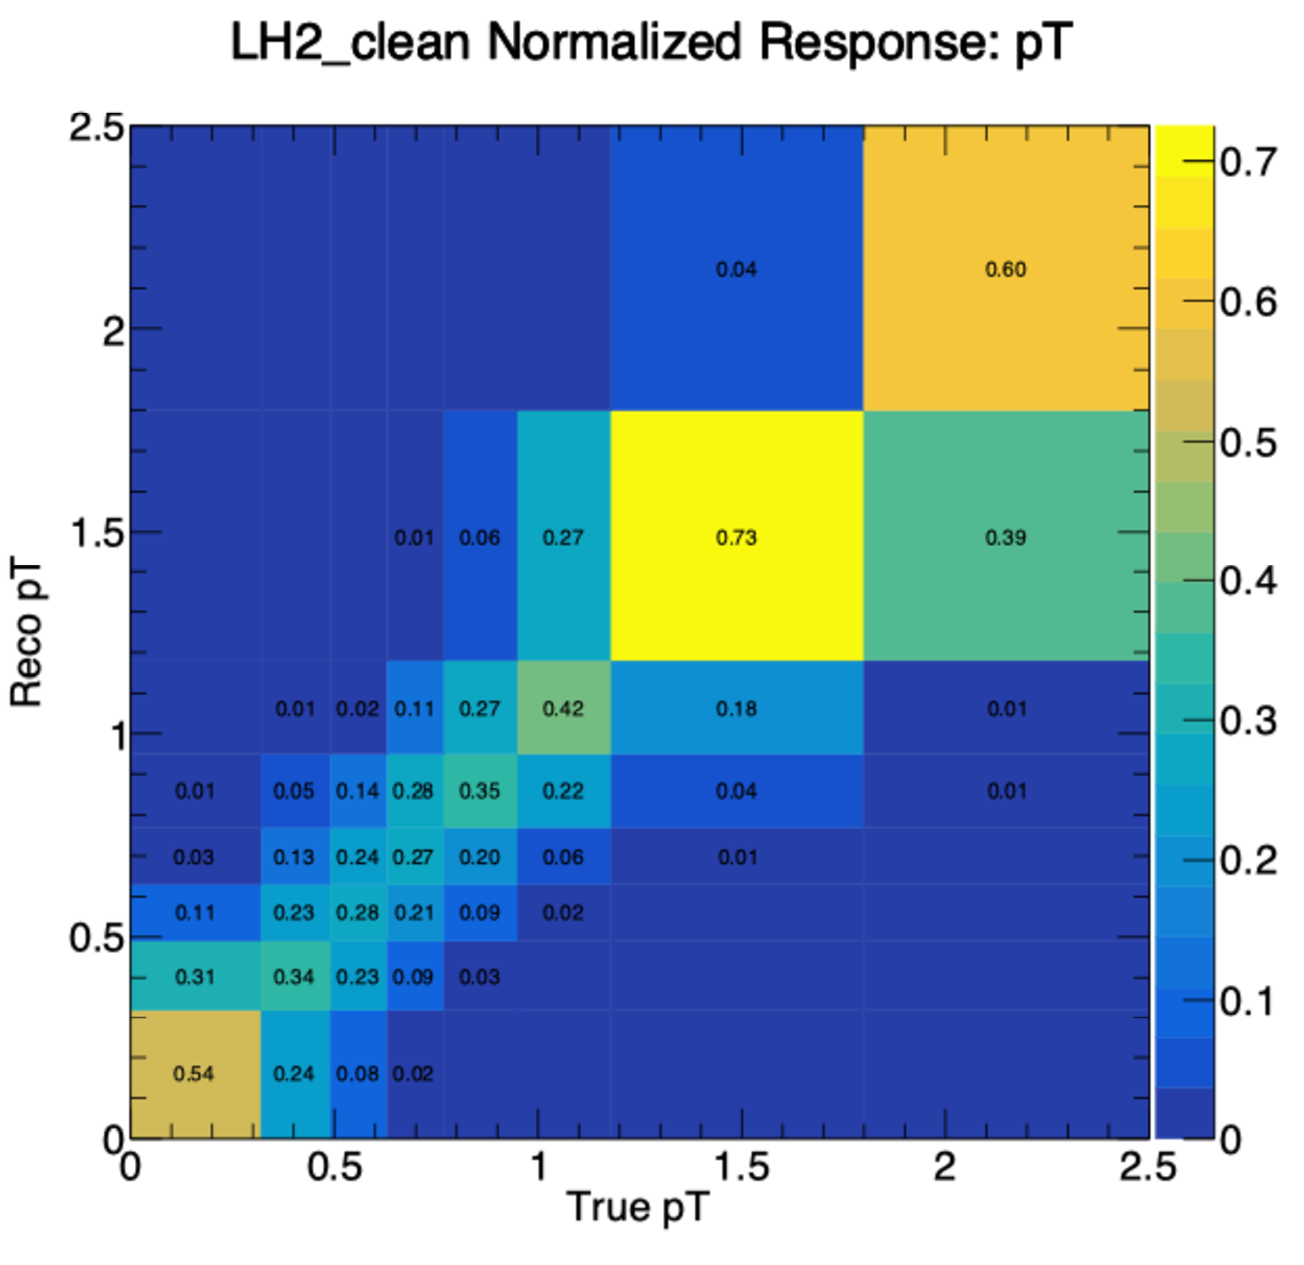
\includegraphics[width=\textwidth,height=0.75\textheight,keepaspectratio]{Response_LH2_Clean.pdf}
        \end{column}
        \begin{column}{0.5\textwidth}
            \centering
            \textbf{LD2 Target}\\
            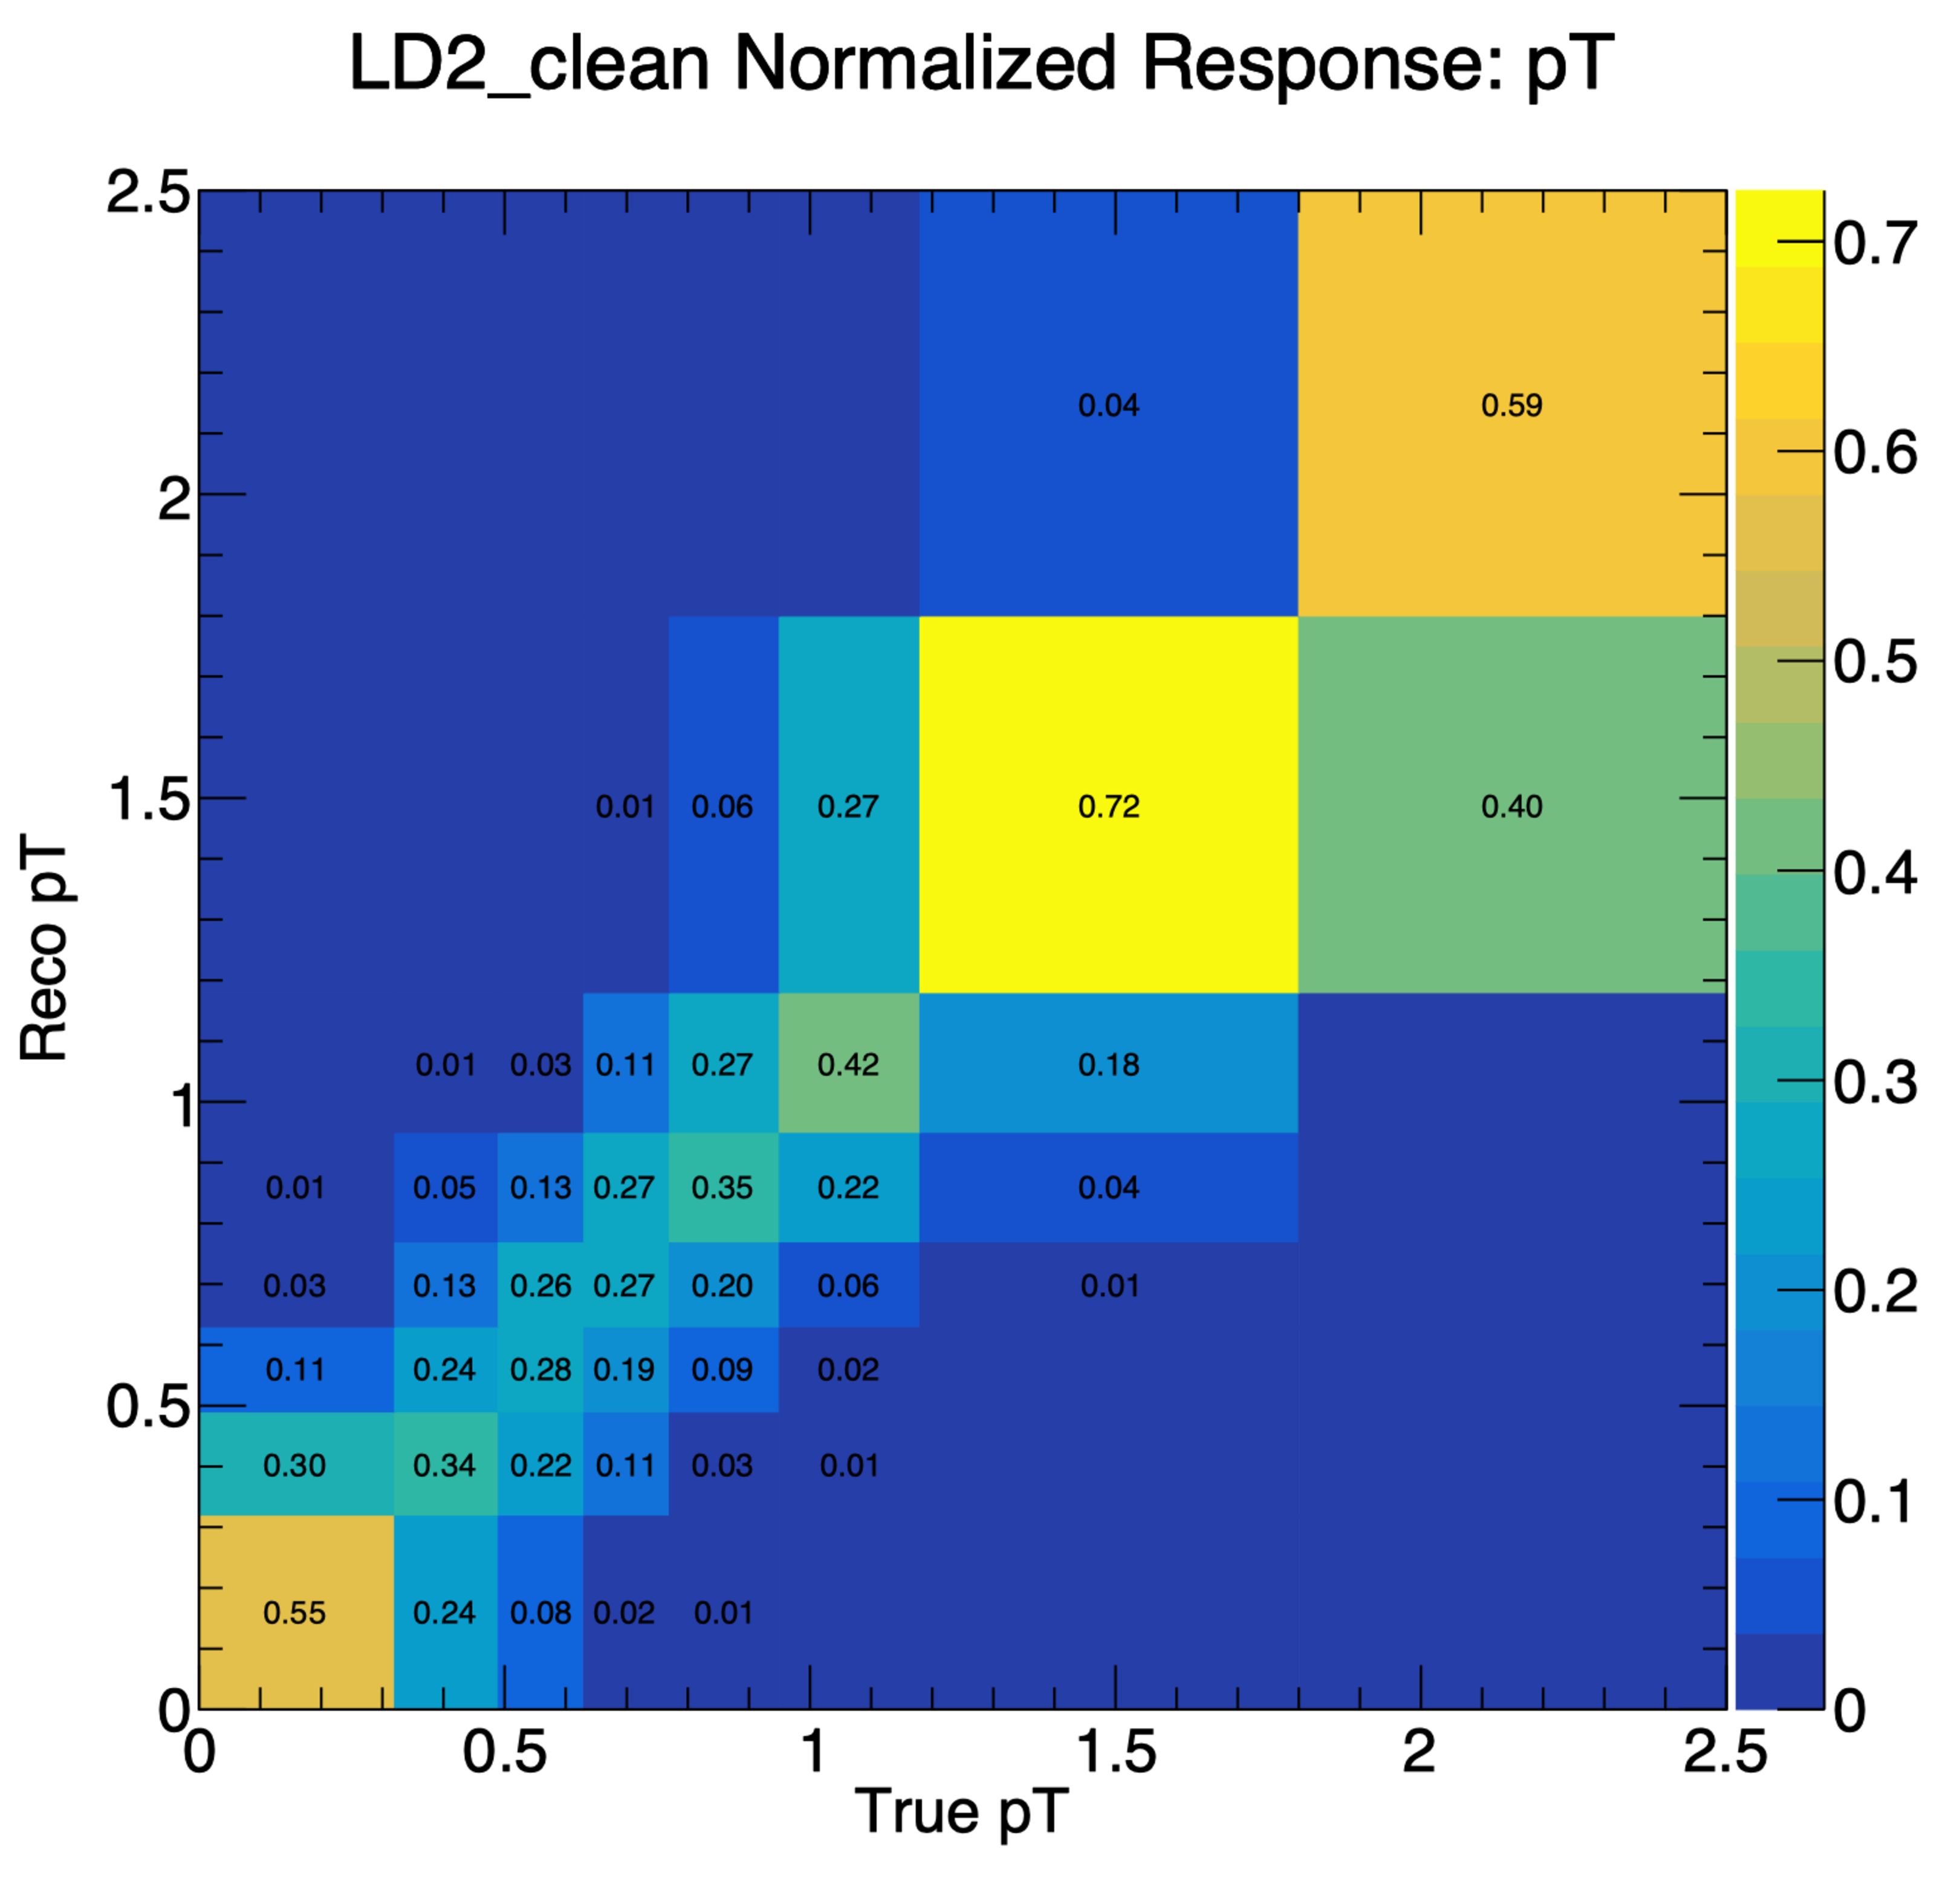
\includegraphics[width=\textwidth,height=0.75\textheight,keepaspectratio]{Response_LD2_Clean.pdf}
        \end{column}
    \end{columns}
\end{frame}

% --- RESPONSE MATRICES (MESSY) ---
\begin{frame}{Response Matrices (messy)}
    \begin{columns}
        \begin{column}{0.5\textwidth}
            \centering
            \textbf{LH2 Target}\\
            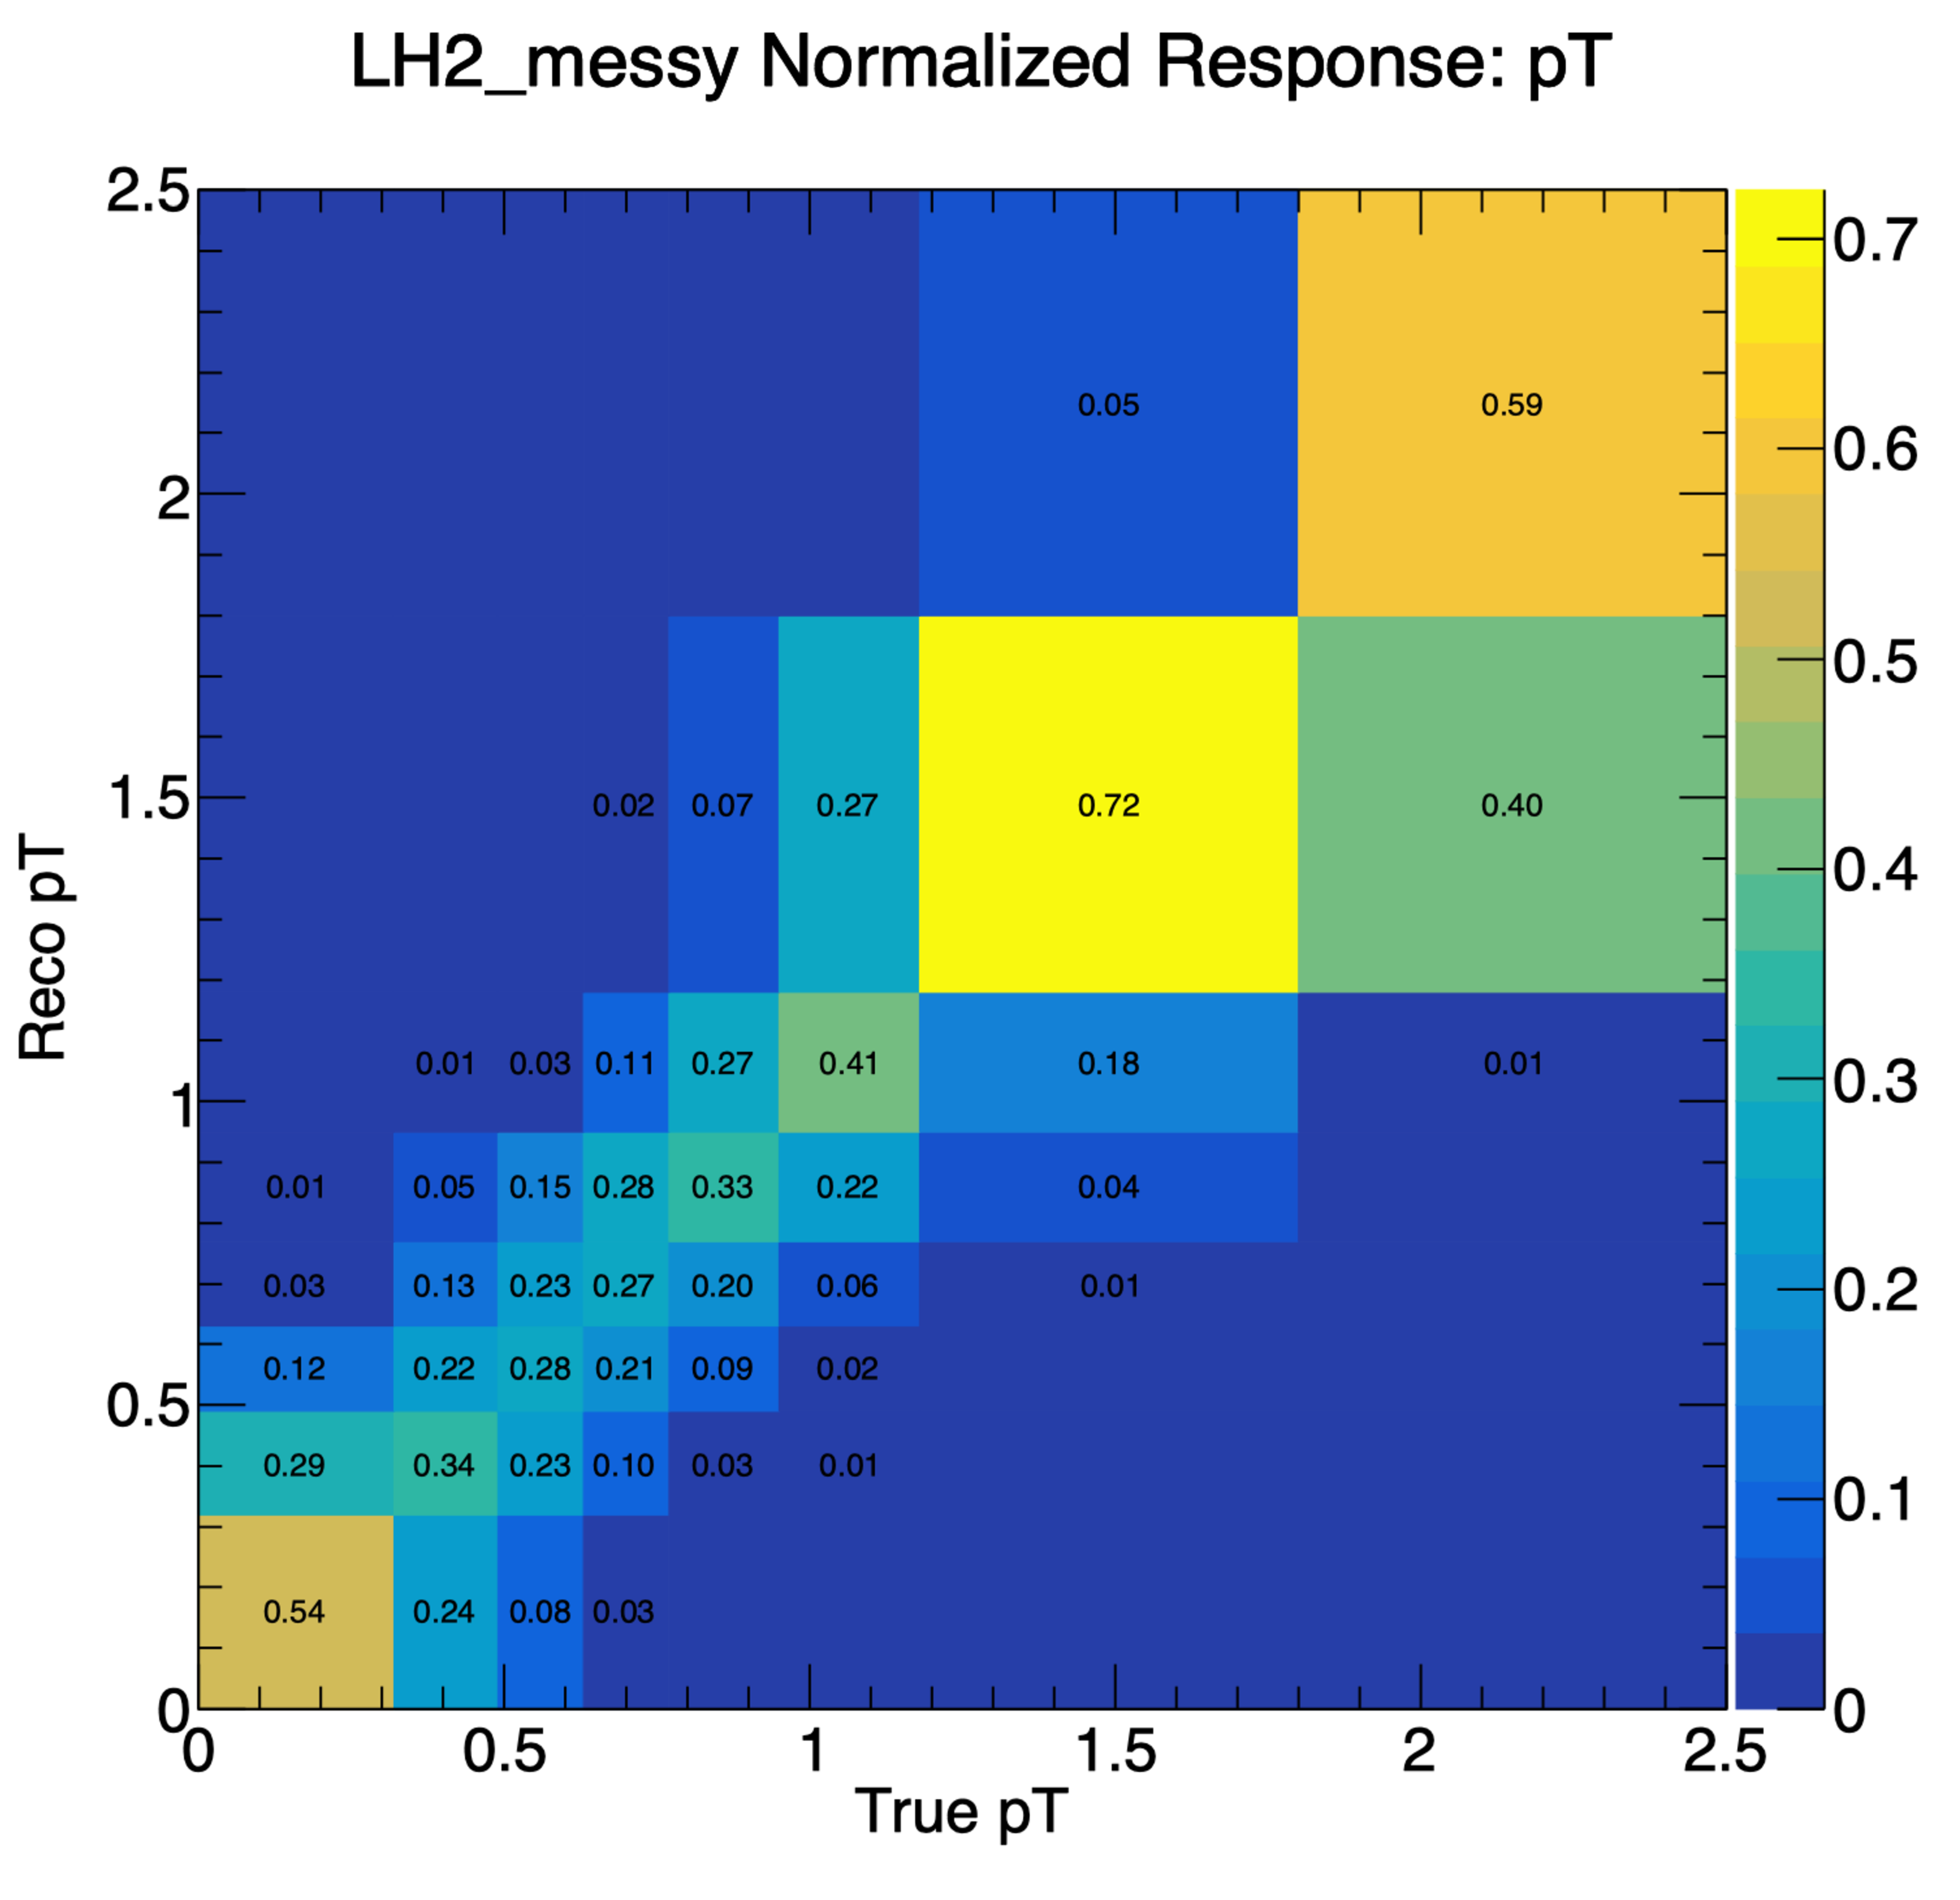
\includegraphics[width=\textwidth,height=0.75\textheight,keepaspectratio]{Response_LH2_Messy.pdf}
        \end{column}
        \begin{column}{0.5\textwidth}
            \centering
            \textbf{LD2 Target}\\
            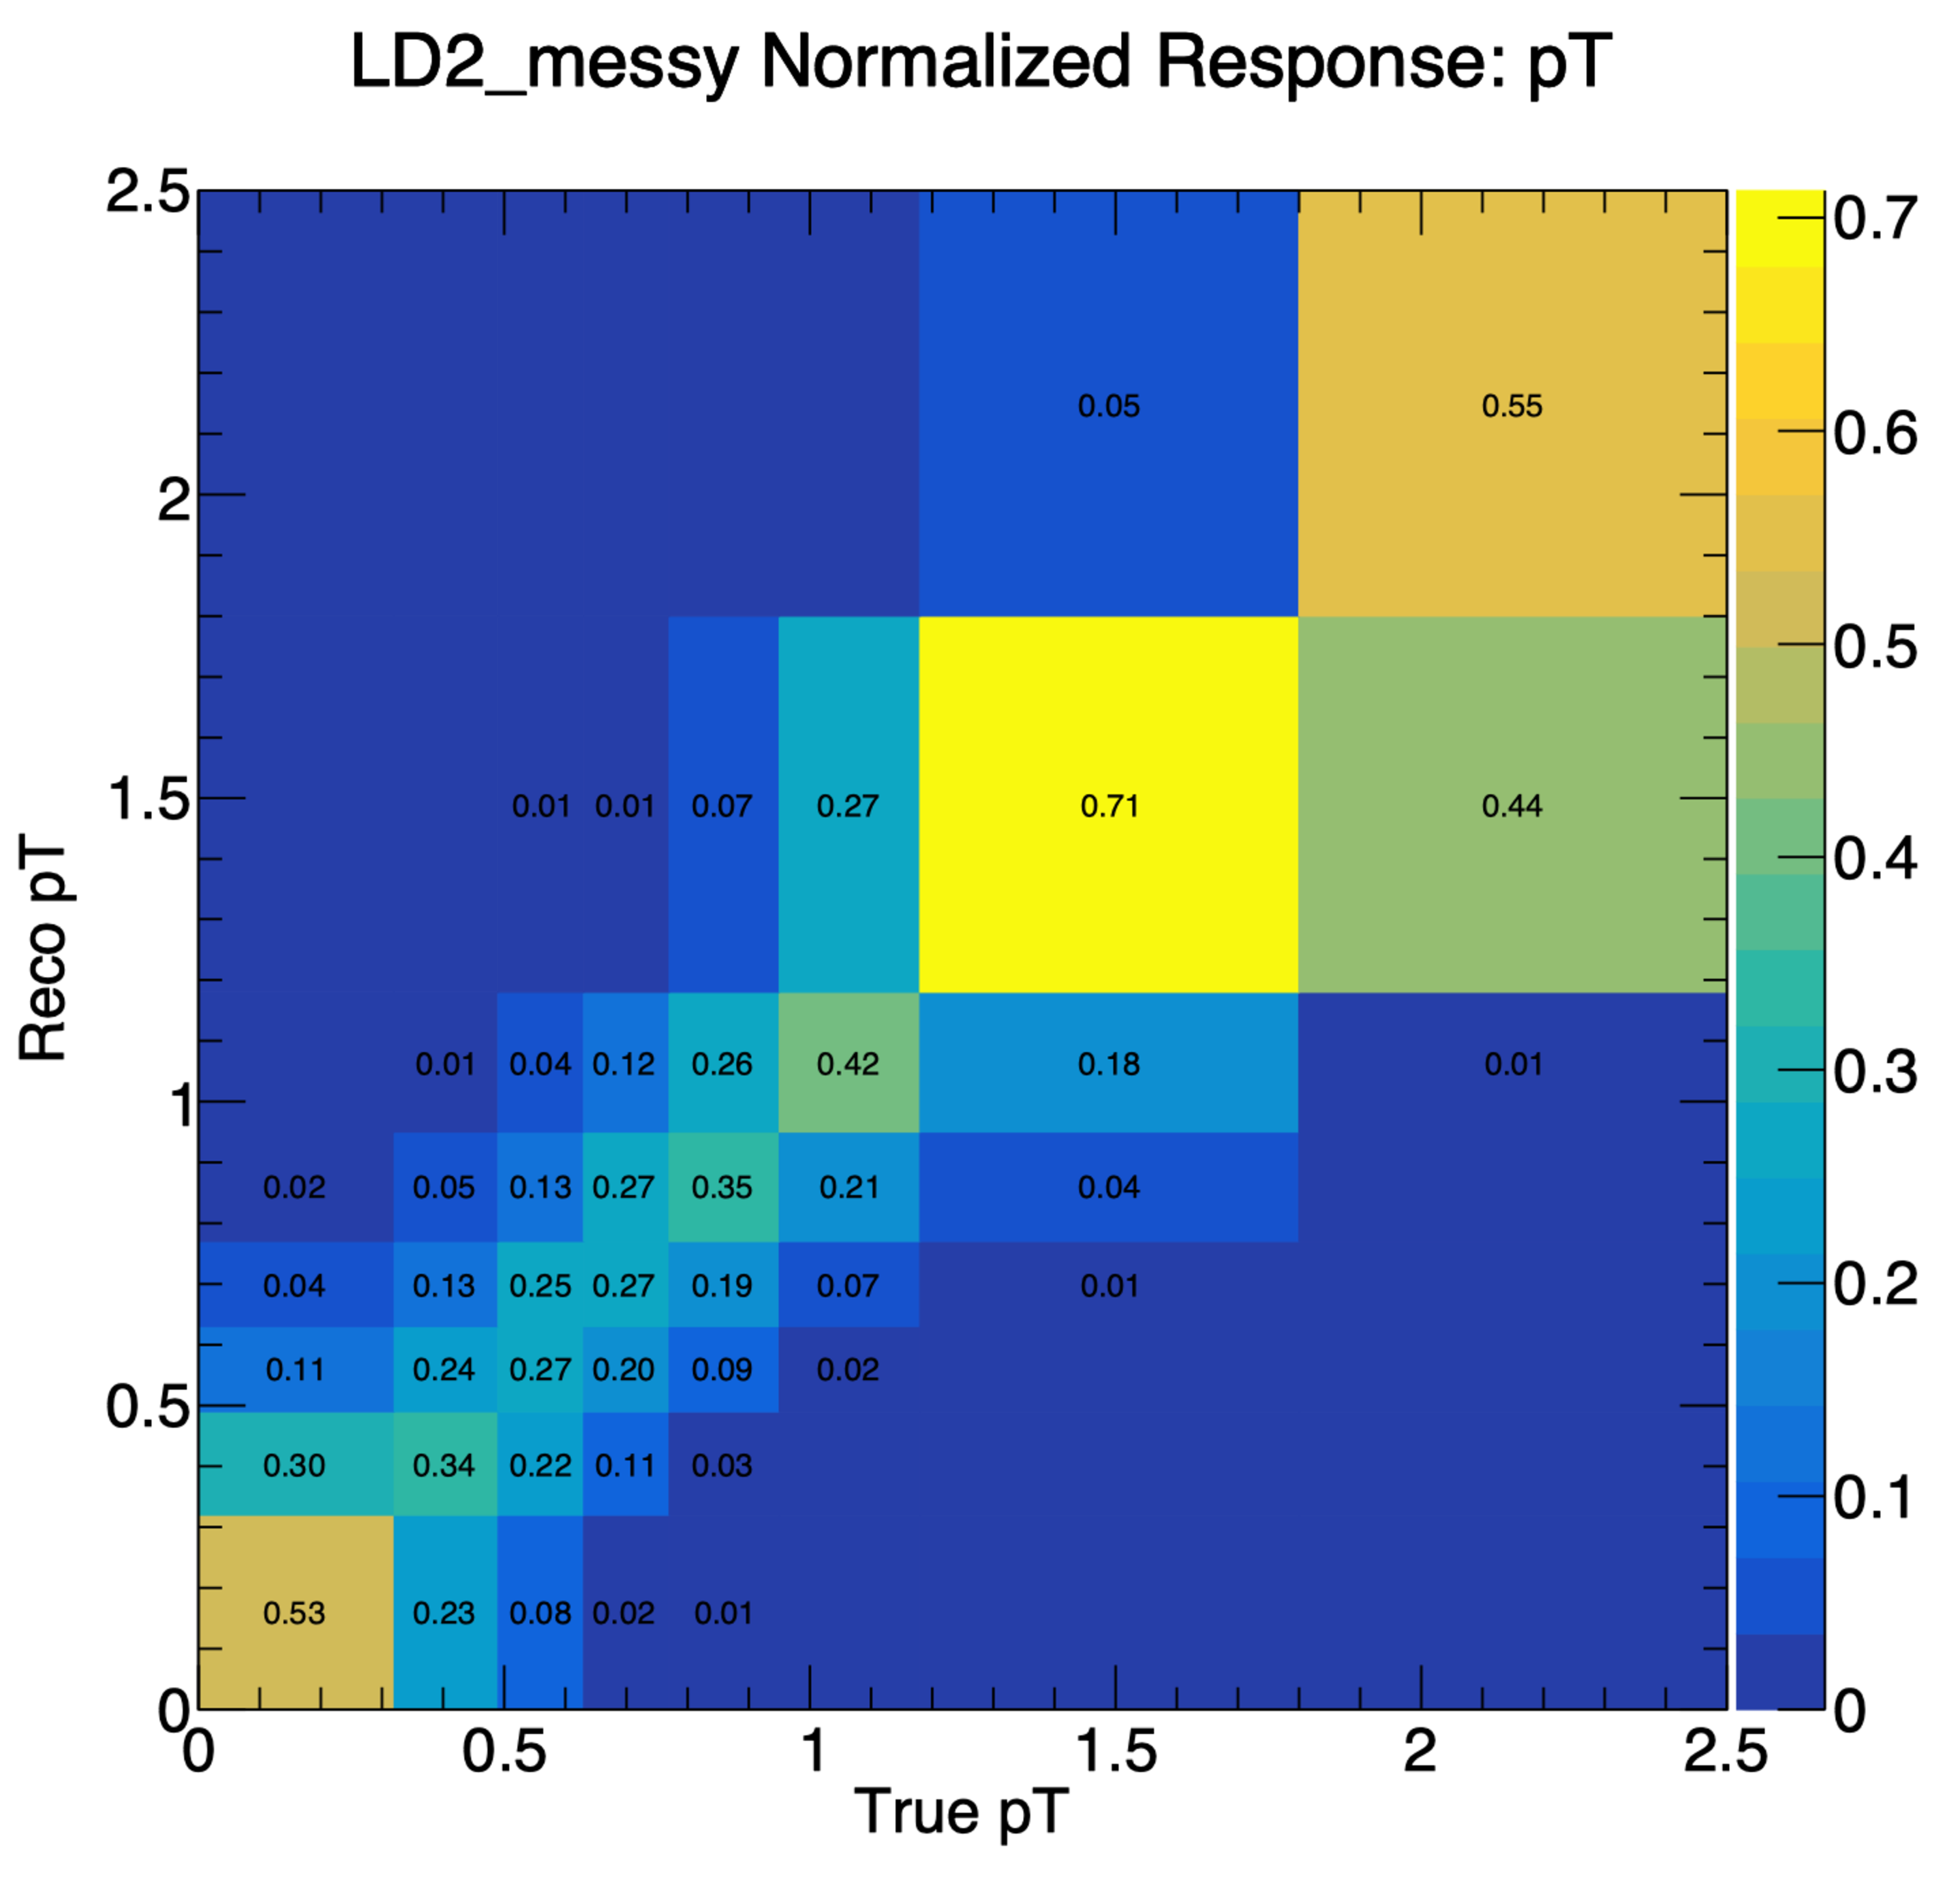
\includegraphics[width=\textwidth,height=0.75\textheight,keepaspectratio]{Response_LD2_Messy.pdf}
        \end{column}
    \end{columns}
\end{frame}

% --- SINGLE DIFFERENTIAL CROSS SECTION SLIDE ---
\begin{frame}{Unfolded Single Differential Cross-Section as a function of $p_T$}
    \begin{columns}
        \begin{column}{0.5\textwidth}
            \centering
            \textbf{LH2 Target}\\
            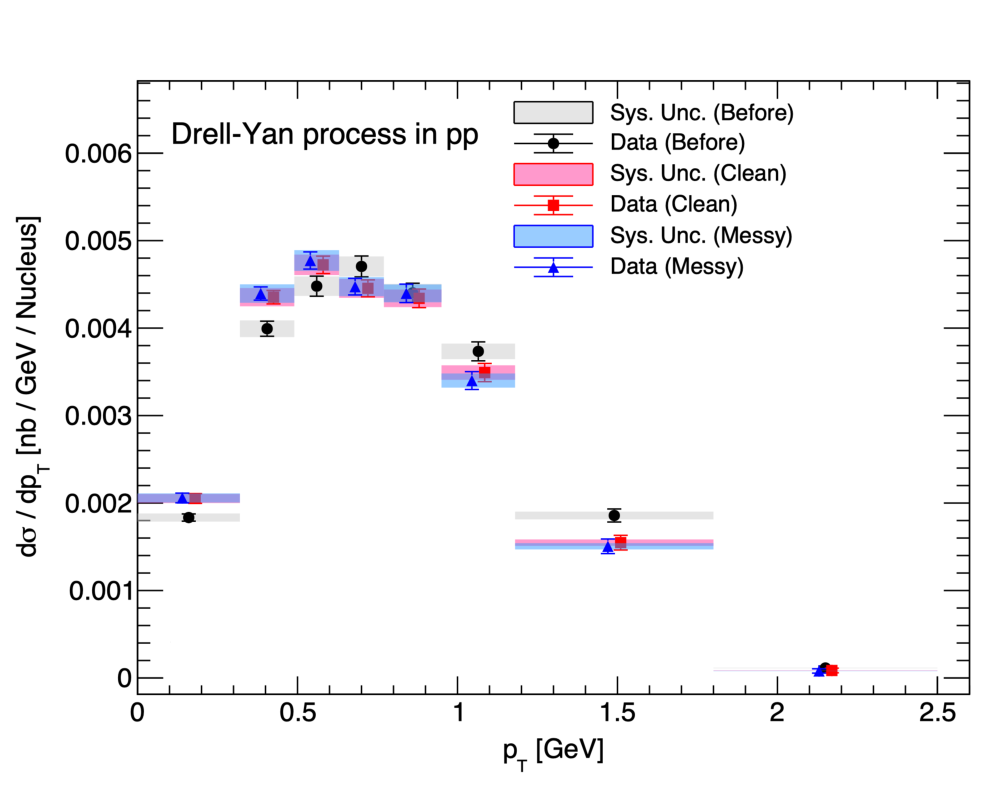
\includegraphics[width=\textwidth,height=0.75\textheight,keepaspectratio]{SingleDifferentialCross-Section_pp.pdf}
        \end{column}
        \begin{column}{0.5\textwidth}
            \centering
            \textbf{LD2 Target}\\
            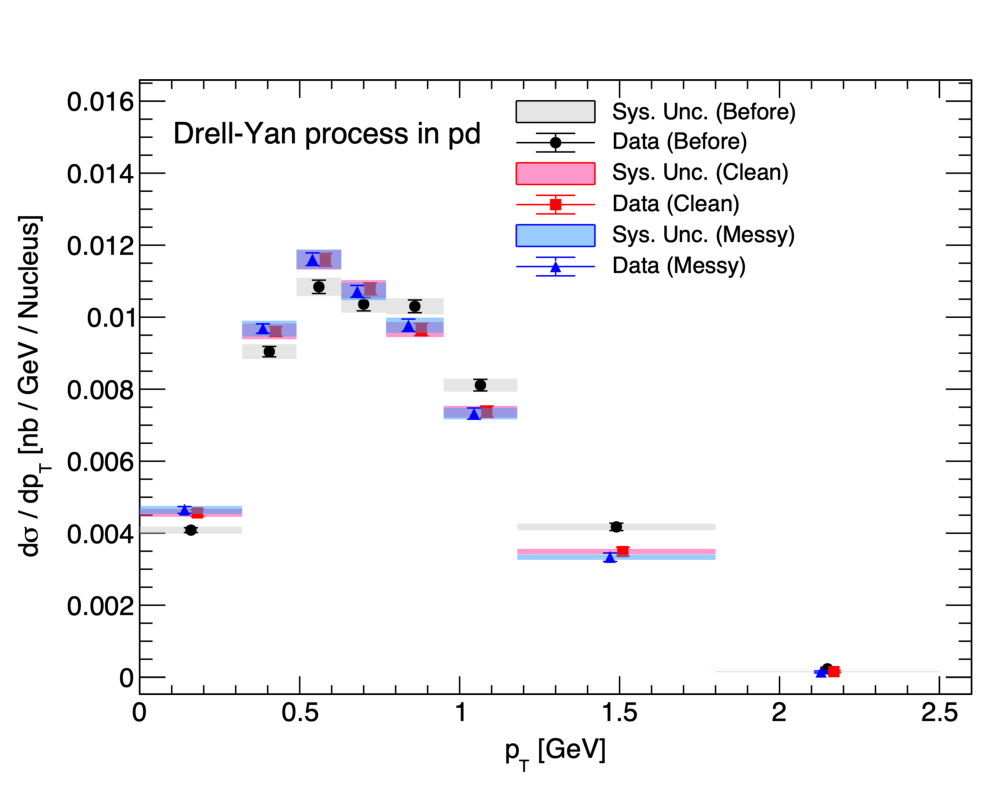
\includegraphics[width=\textwidth,height=0.75\textheight,keepaspectratio]{SingleDifferentialCross-Section_pd.pdf}
        \end{column}
    \end{columns}
\end{frame}

\begin{frame}{-0.05 $\leq x_F <$ 0.00}
    \begin{columns}
        \begin{column}{0.5\textwidth}
            \centering
            \textbf{LH2 Target}\\
            
\includegraphics[width=\textwidth,height=0.75\textheight,keepaspectratio]{CrossSection_LH2_xF_-0.05_0.00_GeoCenter.pdf}
        \end{column}
        \begin{column}{0.5\textwidth}
            \centering
            \textbf{LD2 Target}\\
            
\includegraphics[width=\textwidth,height=0.75\textheight,keepaspectratio]{CrossSection_LD2_xF_-0.05_0.00_GeoCenter.pdf}
        \end{column}
    \end{columns}
\end{frame}

\begin{frame}{0.00 $\leq x_F <$ 0.05}
    \begin{columns}
        \begin{column}{0.5\textwidth}
            \centering
            \textbf{LH2 Target}\\
            
\includegraphics[width=\textwidth,height=0.75\textheight,keepaspectratio]{CrossSection_LH2_xF_0.00_0.05_GeoCenter.pdf}
        \end{column}
        \begin{column}{0.5\textwidth}
            \centering
            \textbf{LD2 Target}\\
            
\includegraphics[width=\textwidth,height=0.75\textheight,keepaspectratio]{CrossSection_LD2_xF_0.00_0.05_GeoCenter.pdf}
        \end{column}
    \end{columns}
\end{frame}

\begin{frame}{0.05 $\leq x_F <$ 0.10}
    \begin{columns}
        \begin{column}{0.5\textwidth}
            \centering
            \textbf{LH2 Target}\\
            
\includegraphics[width=\textwidth,height=0.75\textheight,keepaspectratio]{CrossSection_LH2_xF_0.05_0.10_GeoCenter.pdf}
        \end{column}
        \begin{column}{0.5\textwidth}
            \centering
            \textbf{LD2 Target}\\
            
\includegraphics[width=\textwidth,height=0.75\textheight,keepaspectratio]{CrossSection_LD2_xF_0.05_0.10_GeoCenter.pdf}
        \end{column}
    \end{columns}
\end{frame}

\begin{frame}{0.10 $\leq x_F <$ 0.15}
    \begin{columns}
        \begin{column}{0.5\textwidth}
            \centering
            \textbf{LH2 Target}\\
            
\includegraphics[width=\textwidth,height=0.75\textheight,keepaspectratio]{CrossSection_LH2_xF_0.10_0.15_GeoCenter.pdf}
        \end{column}
        \begin{column}{0.5\textwidth}
            \centering
            \textbf{LD2 Target}\\
            
\includegraphics[width=\textwidth,height=0.75\textheight,keepaspectratio]{CrossSection_LD2_xF_0.10_0.15_GeoCenter.pdf}
        \end{column}
    \end{columns}
\end{frame}

\begin{frame}{0.15 $\leq x_F <$ 0.20}
    \begin{columns}
        \begin{column}{0.5\textwidth}
            \centering
            \textbf{LH2 Target}\\
            
\includegraphics[width=\textwidth,height=0.75\textheight,keepaspectratio]{CrossSection_LH2_xF_0.15_0.20_GeoCenter.pdf}
        \end{column}
        \begin{column}{0.5\textwidth}
            \centering
            \textbf{LD2 Target}\\
            
\includegraphics[width=\textwidth,height=0.75\textheight,keepaspectratio]{CrossSection_LD2_xF_0.15_0.20_GeoCenter.pdf}
        \end{column}
    \end{columns}
\end{frame}

\begin{frame}{0.20 $\leq x_F <$ 0.25}
    \begin{columns}
        \begin{column}{0.5\textwidth}
            \centering
            \textbf{LH2 Target}\\
            
\includegraphics[width=\textwidth,height=0.75\textheight,keepaspectratio]{CrossSection_LH2_xF_0.20_0.25_GeoCenter.pdf}
        \end{column}
        \begin{column}{0.5\textwidth}
            \centering
            \textbf{LD2 Target}\\
            
\includegraphics[width=\textwidth,height=0.75\textheight,keepaspectratio]{CrossSection_LD2_xF_0.20_0.25_GeoCenter.pdf}
        \end{column}
    \end{columns}
\end{frame}

\begin{frame}{0.25 $\leq x_F <$ 0.30}
    \begin{columns}
        \begin{column}{0.5\textwidth}
            \centering
            \textbf{LH2 Target}\\
            
\includegraphics[width=\textwidth,height=0.75\textheight,keepaspectratio]{CrossSection_LH2_xF_0.25_0.30_GeoCenter.pdf}
        \end{column}
        \begin{column}{0.5\textwidth}
            \centering
            \textbf{LD2 Target}\\
            
\includegraphics[width=\textwidth,height=0.75\textheight,keepaspectratio]{CrossSection_LD2_xF_0.25_0.30_GeoCenter.pdf}
        \end{column}
    \end{columns}
\end{frame}

\begin{frame}{0.30 $\leq x_F <$ 0.35}
    \begin{columns}
        \begin{column}{0.5\textwidth}
            \centering
            \textbf{LH2 Target}\\
            
\includegraphics[width=\textwidth,height=0.75\textheight,keepaspectratio]{CrossSection_LH2_xF_0.30_0.35_GeoCenter.pdf}
        \end{column}
        \begin{column}{0.5\textwidth}
            \centering
            \textbf{LD2 Target}\\
            
\includegraphics[width=\textwidth,height=0.75\textheight,keepaspectratio]{CrossSection_LD2_xF_0.30_0.35_GeoCenter.pdf}
        \end{column}
    \end{columns}
\end{frame}

\begin{frame}{0.35 $\leq x_F <$ 0.40}
    \begin{columns}
        \begin{column}{0.5\textwidth}
            \centering
            \textbf{LH2 Target}\\
            
\includegraphics[width=\textwidth,height=0.75\textheight,keepaspectratio]{CrossSection_LH2_xF_0.35_0.40_GeoCenter.pdf}
        \end{column}
        \begin{column}{0.5\textwidth}
            \centering
            \textbf{LD2 Target}\\
            
\includegraphics[width=\textwidth,height=0.75\textheight,keepaspectratio]{CrossSection_LD2_xF_0.35_0.40_GeoCenter.pdf}
        \end{column}
    \end{columns}
\end{frame}

\begin{frame}{0.40 $\leq x_F <$ 0.45}
    \begin{columns}
        \begin{column}{0.5\textwidth}
            \centering
            \textbf{LH2 Target}\\
            
\includegraphics[width=\textwidth,height=0.75\textheight,keepaspectratio]{CrossSection_LH2_xF_0.40_0.45_GeoCenter.pdf}
        \end{column}
        \begin{column}{0.5\textwidth}
            \centering
            \textbf{LD2 Target}\\
            
\includegraphics[width=\textwidth,height=0.75\textheight,keepaspectratio]{CrossSection_LD2_xF_0.40_0.45_GeoCenter.pdf}
        \end{column}
    \end{columns}
\end{frame}

\begin{frame}{0.45 $\leq x_F <$ 0.50}
    \begin{columns}
        \begin{column}{0.5\textwidth}
            \centering
            \textbf{LH2 Target}\\
            
\includegraphics[width=\textwidth,height=0.75\textheight,keepaspectratio]{CrossSection_LH2_xF_0.45_0.50_GeoCenter.pdf}
        \end{column}
        \begin{column}{0.5\textwidth}
            \centering
            \textbf{LD2 Target}\\
            
\includegraphics[width=\textwidth,height=0.75\textheight,keepaspectratio]{CrossSection_LD2_xF_0.45_0.50_GeoCenter.pdf}
        \end{column}
    \end{columns}
\end{frame}

\begin{frame}{0.50 $\leq x_F <$ 0.55}
    \begin{columns}
        \begin{column}{0.5\textwidth}
            \centering
            \textbf{LH2 Target}\\
            
\includegraphics[width=\textwidth,height=0.75\textheight,keepaspectratio]{CrossSection_LH2_xF_0.50_0.55_GeoCenter.pdf}
        \end{column}
        \begin{column}{0.5\textwidth}
            \centering
            \textbf{LD2 Target}\\
            
\includegraphics[width=\textwidth,height=0.75\textheight,keepaspectratio]{CrossSection_LD2_xF_0.50_0.55_GeoCenter.pdf}
        \end{column}
    \end{columns}
\end{frame}

\begin{frame}{0.55 $\leq x_F <$ 0.60}
    \begin{columns}
        \begin{column}{0.5\textwidth}
            \centering
            \textbf{LH2 Target}\\
            
\includegraphics[width=\textwidth,height=0.75\textheight,keepaspectratio]{CrossSection_LH2_xF_0.55_0.60_GeoCenter.pdf}
        \end{column}
        \begin{column}{0.5\textwidth}
            \centering
            \textbf{LD2 Target}\\
            
\includegraphics[width=\textwidth,height=0.75\textheight,keepaspectratio]{CrossSection_LD2_xF_0.55_0.60_GeoCenter.pdf}
        \end{column}
    \end{columns}
\end{frame}

\begin{frame}{0.60 $\leq x_F <$ 0.65}
    \begin{columns}
        \begin{column}{0.5\textwidth}
            \centering
            \textbf{LH2 Target}\\
            
\includegraphics[width=\textwidth,height=0.75\textheight,keepaspectratio]{CrossSection_LH2_xF_0.60_0.65_GeoCenter.pdf}
        \end{column}
        \begin{column}{0.5\textwidth}
            \centering
            \textbf{LD2 Target}\\
            
\includegraphics[width=\textwidth,height=0.75\textheight,keepaspectratio]{CrossSection_LD2_xF_0.60_0.65_GeoCenter.pdf}
        \end{column}
    \end{columns}
\end{frame}

\begin{frame}{0.65 $\leq x_F <$ 0.70}
    \begin{columns}
        \begin{column}{0.5\textwidth}
            \centering
            \textbf{LH2 Target}\\
            
\includegraphics[width=\textwidth,height=0.75\textheight,keepaspectratio]{CrossSection_LH2_xF_0.65_0.70_GeoCenter.pdf}
        \end{column}
        \begin{column}{0.5\textwidth}
            \centering
            \textbf{LD2 Target}\\
            
\includegraphics[width=\textwidth,height=0.75\textheight,keepaspectratio]{CrossSection_LD2_xF_0.65_0.70_GeoCenter.pdf}
        \end{column}
    \end{columns}
\end{frame}

\begin{frame}{0.70 $\leq x_F <$ 0.75}
    \begin{columns}
        \begin{column}{0.5\textwidth}
            \centering
            \textbf{LH2 Target}\\
            
\includegraphics[width=\textwidth,height=0.75\textheight,keepaspectratio]{CrossSection_LH2_xF_0.70_0.75_GeoCenter.pdf}
        \end{column}
        \begin{column}{0.5\textwidth}
            \centering
            \textbf{LD2 Target}\\
            
\includegraphics[width=\textwidth,height=0.75\textheight,keepaspectratio]{CrossSection_LD2_xF_0.70_0.75_GeoCenter.pdf}
        \end{column}
    \end{columns}
\end{frame}

\begin{frame}{0.75 $\leq x_F <$ 0.80}
    \begin{columns}
        \begin{column}{0.5\textwidth}
            \centering
            \textbf{LH2 Target}\\
            
\includegraphics[width=\textwidth,height=0.75\textheight,keepaspectratio]{CrossSection_LH2_xF_0.75_0.80_GeoCenter.pdf}
        \end{column}
        \begin{column}{0.5\textwidth}
            \centering
            \textbf{LD2 Target}\\
            
\includegraphics[width=\textwidth,height=0.75\textheight,keepaspectratio]{CrossSection_LD2_xF_0.75_0.80_GeoCenter.pdf}
        \end{column}
    \end{columns}
\end{frame}

\begin{frame}{0.80 $\leq x_F <$ 0.85}
    \begin{columns}
        \begin{column}{0.5\textwidth}
            \centering
            \textbf{LH2 Target}\\
            
\includegraphics[width=\textwidth,height=0.75\textheight,keepaspectratio]{CrossSection_LH2_xF_0.80_0.85_GeoCenter.pdf}
        \end{column}
        \begin{column}{0.5\textwidth}
            \centering
            \textbf{LD2 Target}\\
            
\includegraphics[width=\textwidth,height=0.75\textheight,keepaspectratio]{CrossSection_LD2_xF_0.80_0.85_GeoCenter.pdf}
        \end{column}
    \end{columns}
\end{frame}

\begin{frame}{Conclusions and Next Steps}
    \begin{itemize}
        \setlength\itemsep{1em}
        \item Unfolding calculation was added for double differential cross-section successfully
        \item Need to recalculate acceptance correction for Runs: [2, 3] separately (Kenichi and Harsha are working on it)
        \item Finalizing the draft for the publication and requesting collaboration approval
    \end{itemize}
\end{frame}

\appendix
\begin{frame}[plain,c]
    \begin{center}
        \Huge \textbf{Backup Slides: Unfolding Optimization}
    \end{center}
\end{frame}

\begin{frame}{Opt (Messy): -0.05 $\leq x_F <$ 0.00}
    \begin{columns}
        \begin{column}{0.5\textwidth}
            \centering
            \textbf{LH2 (Messy)}\\
            
\includegraphics[width=\textwidth,height=0.75\textheight,keepaspectratio]{Unfolding_Optimization_LH2_Messy_xF_0.pdf}
        \end{column}
        \begin{column}{0.5\textwidth}
            \centering
            \textbf{LD2 (Messy)}\\
            
\includegraphics[width=\textwidth,height=0.75\textheight,keepaspectratio]{Unfolding_Optimization_LD2_Messy_xF_0.pdf}
        \end{column}
    \end{columns}
\end{frame}

\begin{frame}{Opt (Messy): 0.00 $\leq x_F <$ 0.05}
    \begin{columns}
        \begin{column}{0.5\textwidth}
            \centering
            \textbf{LH2 (Messy)}\\
            
\includegraphics[width=\textwidth,height=0.75\textheight,keepaspectratio]{Unfolding_Optimization_LH2_Messy_xF_1.pdf}
        \end{column}
        \begin{column}{0.5\textwidth}
            \centering
            \textbf{LD2 (Messy)}\\
            
\includegraphics[width=\textwidth,height=0.75\textheight,keepaspectratio]{Unfolding_Optimization_LD2_Messy_xF_1.pdf}
        \end{column}
    \end{columns}
\end{frame}

\begin{frame}{Opt (Messy): 0.05 $\leq x_F <$ 0.10}
    \begin{columns}
        \begin{column}{0.5\textwidth}
            \centering
            \textbf{LH2 (Messy)}\\
            
\includegraphics[width=\textwidth,height=0.75\textheight,keepaspectratio]{Unfolding_Optimization_LH2_Messy_xF_2.pdf}
        \end{column}
        \begin{column}{0.5\textwidth}
            \centering
            \textbf{LD2 (Messy)}\\
            
\includegraphics[width=\textwidth,height=0.75\textheight,keepaspectratio]{Unfolding_Optimization_LD2_Messy_xF_2.pdf}
        \end{column}
    \end{columns}
\end{frame}

\begin{frame}{Opt (Messy): 0.10 $\leq x_F <$ 0.15}
    \begin{columns}
        \begin{column}{0.5\textwidth}
            \centering
            \textbf{LH2 (Messy)}\\
            
\includegraphics[width=\textwidth,height=0.75\textheight,keepaspectratio]{Unfolding_Optimization_LH2_Messy_xF_3.pdf}
        \end{column}
        \begin{column}{0.5\textwidth}
            \centering
            \textbf{LD2 (Messy)}\\
            
\includegraphics[width=\textwidth,height=0.75\textheight,keepaspectratio]{Unfolding_Optimization_LD2_Messy_xF_3.pdf}
        \end{column}
    \end{columns}
\end{frame}

\begin{frame}{Opt (Messy): 0.15 $\leq x_F <$ 0.20}
    \begin{columns}
        \begin{column}{0.5\textwidth}
            \centering
            \textbf{LH2 (Messy)}\\
            
\includegraphics[width=\textwidth,height=0.75\textheight,keepaspectratio]{Unfolding_Optimization_LH2_Messy_xF_4.pdf}
        \end{column}
        \begin{column}{0.5\textwidth}
            \centering
            \textbf{LD2 (Messy)}\\
            
\includegraphics[width=\textwidth,height=0.75\textheight,keepaspectratio]{Unfolding_Optimization_LD2_Messy_xF_4.pdf}
        \end{column}
    \end{columns}
\end{frame}

\begin{frame}{Opt (Messy): 0.20 $\leq x_F <$ 0.25}
    \begin{columns}
        \begin{column}{0.5\textwidth}
            \centering
            \textbf{LH2 (Messy)}\\
            
\includegraphics[width=\textwidth,height=0.75\textheight,keepaspectratio]{Unfolding_Optimization_LH2_Messy_xF_5.pdf}
        \end{column}
        \begin{column}{0.5\textwidth}
            \centering
            \textbf{LD2 (Messy)}\\
            
\includegraphics[width=\textwidth,height=0.75\textheight,keepaspectratio]{Unfolding_Optimization_LD2_Messy_xF_5.pdf}
        \end{column}
    \end{columns}
\end{frame}

\begin{frame}{Opt (Messy): 0.25 $\leq x_F <$ 0.30}
    \begin{columns}
        \begin{column}{0.5\textwidth}
            \centering
            \textbf{LH2 (Messy)}\\
            
\includegraphics[width=\textwidth,height=0.75\textheight,keepaspectratio]{Unfolding_Optimization_LH2_Messy_xF_6.pdf}
        \end{column}
        \begin{column}{0.5\textwidth}
            \centering
            \textbf{LD2 (Messy)}\\
            
\includegraphics[width=\textwidth,height=0.75\textheight,keepaspectratio]{Unfolding_Optimization_LD2_Messy_xF_6.pdf}
        \end{column}
    \end{columns}
\end{frame}

\begin{frame}{Opt (Messy): 0.30 $\leq x_F <$ 0.35}
    \begin{columns}
        \begin{column}{0.5\textwidth}
            \centering
            \textbf{LH2 (Messy)}\\
            
\includegraphics[width=\textwidth,height=0.75\textheight,keepaspectratio]{Unfolding_Optimization_LH2_Messy_xF_7.pdf}
        \end{column}
        \begin{column}{0.5\textwidth}
            \centering
            \textbf{LD2 (Messy)}\\
            
\includegraphics[width=\textwidth,height=0.75\textheight,keepaspectratio]{Unfolding_Optimization_LD2_Messy_xF_7.pdf}
        \end{column}
    \end{columns}
\end{frame}

\begin{frame}{Opt (Messy): 0.35 $\leq x_F <$ 0.40}
    \begin{columns}
        \begin{column}{0.5\textwidth}
            \centering
            \textbf{LH2 (Messy)}\\
            
\includegraphics[width=\textwidth,height=0.75\textheight,keepaspectratio]{Unfolding_Optimization_LH2_Messy_xF_8.pdf}
        \end{column}
        \begin{column}{0.5\textwidth}
            \centering
            \textbf{LD2 (Messy)}\\
            
\includegraphics[width=\textwidth,height=0.75\textheight,keepaspectratio]{Unfolding_Optimization_LD2_Messy_xF_8.pdf}
        \end{column}
    \end{columns}
\end{frame}

\begin{frame}{Opt (Messy): 0.40 $\leq x_F <$ 0.45}
    \begin{columns}
        \begin{column}{0.5\textwidth}
            \centering
            \textbf{LH2 (Messy)}\\
            
\includegraphics[width=\textwidth,height=0.75\textheight,keepaspectratio]{Unfolding_Optimization_LH2_Messy_xF_9.pdf}
        \end{column}
        \begin{column}{0.5\textwidth}
            \centering
            \textbf{LD2 (Messy)}\\
            
\includegraphics[width=\textwidth,height=0.75\textheight,keepaspectratio]{Unfolding_Optimization_LD2_Messy_xF_9.pdf}
        \end{column}
    \end{columns}
\end{frame}

\begin{frame}{Opt (Messy): 0.45 $\leq x_F <$ 0.50}
    \begin{columns}
        \begin{column}{0.5\textwidth}
            \centering
            \textbf{LH2 (Messy)}\\
            
\includegraphics[width=\textwidth,height=0.75\textheight,keepaspectratio]{Unfolding_Optimization_LH2_Messy_xF_10.pdf}
        \end{column}
        \begin{column}{0.5\textwidth}
            \centering
            \textbf{LD2 (Messy)}\\
            
\includegraphics[width=\textwidth,height=0.75\textheight,keepaspectratio]{Unfolding_Optimization_LD2_Messy_xF_10.pdf}
        \end{column}
    \end{columns}
\end{frame}

\begin{frame}{Opt (Messy): 0.50 $\leq x_F <$ 0.55}
    \begin{columns}
        \begin{column}{0.5\textwidth}
            \centering
            \textbf{LH2 (Messy)}\\
            
\includegraphics[width=\textwidth,height=0.75\textheight,keepaspectratio]{Unfolding_Optimization_LH2_Messy_xF_11.pdf}
        \end{column}
        \begin{column}{0.5\textwidth}
            \centering
            \textbf{LD2 (Messy)}\\
            
\includegraphics[width=\textwidth,height=0.75\textheight,keepaspectratio]{Unfolding_Optimization_LD2_Messy_xF_11.pdf}
        \end{column}
    \end{columns}
\end{frame}

\begin{frame}{Opt (Messy): 0.55 $\leq x_F <$ 0.60}
    \begin{columns}
        \begin{column}{0.5\textwidth}
            \centering
            \textbf{LH2 (Messy)}\\
            
\includegraphics[width=\textwidth,height=0.75\textheight,keepaspectratio]{Unfolding_Optimization_LH2_Messy_xF_12.pdf}
        \end{column}
        \begin{column}{0.5\textwidth}
            \centering
            \textbf{LD2 (Messy)}\\
            
\includegraphics[width=\textwidth,height=0.75\textheight,keepaspectratio]{Unfolding_Optimization_LD2_Messy_xF_12.pdf}
        \end{column}
    \end{columns}
\end{frame}

\begin{frame}{Opt (Messy): 0.60 $\leq x_F <$ 0.65}
    \begin{columns}
        \begin{column}{0.5\textwidth}
            \centering
            \textbf{LH2 (Messy)}\\
            
\includegraphics[width=\textwidth,height=0.75\textheight,keepaspectratio]{Unfolding_Optimization_LH2_Messy_xF_13.pdf}
        \end{column}
        \begin{column}{0.5\textwidth}
            \centering
            \textbf{LD2 (Messy)}\\
            
\includegraphics[width=\textwidth,height=0.75\textheight,keepaspectratio]{Unfolding_Optimization_LD2_Messy_xF_13.pdf}
        \end{column}
    \end{columns}
\end{frame}

\begin{frame}{Opt (Messy): 0.65 $\leq x_F <$ 0.70}
    \begin{columns}
        \begin{column}{0.5\textwidth}
            \centering
            \textbf{LH2 (Messy)}\\
            
\includegraphics[width=\textwidth,height=0.75\textheight,keepaspectratio]{Unfolding_Optimization_LH2_Messy_xF_14.pdf}
        \end{column}
        \begin{column}{0.5\textwidth}
            \centering
            \textbf{LD2 (Messy)}\\
            
\includegraphics[width=\textwidth,height=0.75\textheight,keepaspectratio]{Unfolding_Optimization_LD2_Messy_xF_14.pdf}
        \end{column}
    \end{columns}
\end{frame}

\begin{frame}{Opt (Messy): 0.70 $\leq x_F <$ 0.75}
    \begin{columns}
        \begin{column}{0.5\textwidth}
            \centering
            \textbf{LH2 (Messy)}\\
            
\includegraphics[width=\textwidth,height=0.75\textheight,keepaspectratio]{Unfolding_Optimization_LH2_Messy_xF_15.pdf}
        \end{column}
        \begin{column}{0.5\textwidth}
            \centering
            \textbf{LD2 (Messy)}\\
            
\includegraphics[width=\textwidth,height=0.75\textheight,keepaspectratio]{Unfolding_Optimization_LD2_Messy_xF_15.pdf}
        \end{column}
    \end{columns}
\end{frame}

\begin{frame}{Opt (Messy): 0.75 $\leq x_F <$ 0.80}
    \begin{columns}
        \begin{column}{0.5\textwidth}
            \centering
            \textbf{LH2 (Messy)}\\
            
\includegraphics[width=\textwidth,height=0.75\textheight,keepaspectratio]{Unfolding_Optimization_LH2_Messy_xF_16.pdf}
        \end{column}
        \begin{column}{0.5\textwidth}
            \centering
            \textbf{LD2 (Messy)}\\
            
\includegraphics[width=\textwidth,height=0.75\textheight,keepaspectratio]{Unfolding_Optimization_LD2_Messy_xF_16.pdf}
        \end{column}
    \end{columns}
\end{frame}

\begin{frame}{Opt (Messy): 0.80 $\leq x_F <$ 0.85}
    \begin{columns}
        \begin{column}{0.5\textwidth}
            \centering
            \textbf{LH2 (Messy)}\\
            
\includegraphics[width=\textwidth,height=0.75\textheight,keepaspectratio]{Unfolding_Optimization_LH2_Messy_xF_17.pdf}
        \end{column}
        \begin{column}{0.5\textwidth}
            \centering
            \textbf{LD2 (Messy)}\\
            
\includegraphics[width=\textwidth,height=0.75\textheight,keepaspectratio]{Unfolding_Optimization_LD2_Messy_xF_17.pdf}
        \end{column}
    \end{columns}
\end{frame}

\begin{frame}{Opt (Clean): -0.05 $\leq x_F <$ 0.00}
    \begin{columns}
        \begin{column}{0.5\textwidth}
            \centering
            \textbf{LH2 (Clean)}\\
            
\includegraphics[width=\textwidth,height=0.75\textheight,keepaspectratio]{Unfolding_Optimization_LH2_Clean_xF_0.pdf}
        \end{column}
        \begin{column}{0.5\textwidth}
            \centering
            \textbf{LD2 (Clean)}\\
            
\includegraphics[width=\textwidth,height=0.75\textheight,keepaspectratio]{Unfolding_Optimization_LD2_Clean_xF_0.pdf}
        \end{column}
    \end{columns}
\end{frame}

\begin{frame}{Opt (Clean): 0.00 $\leq x_F <$ 0.05}
    \begin{columns}
        \begin{column}{0.5\textwidth}
            \centering
            \textbf{LH2 (Clean)}\\
            
\includegraphics[width=\textwidth,height=0.75\textheight,keepaspectratio]{Unfolding_Optimization_LH2_Clean_xF_1.pdf}
        \end{column}
        \begin{column}{0.5\textwidth}
            \centering
            \textbf{LD2 (Clean)}\\
            
\includegraphics[width=\textwidth,height=0.75\textheight,keepaspectratio]{Unfolding_Optimization_LD2_Clean_xF_1.pdf}
        \end{column}
    \end{columns}
\end{frame}

\begin{frame}{Opt (Clean): 0.05 $\leq x_F <$ 0.10}
    \begin{columns}
        \begin{column}{0.5\textwidth}
            \centering
            \textbf{LH2 (Clean)}\\
            
\includegraphics[width=\textwidth,height=0.75\textheight,keepaspectratio]{Unfolding_Optimization_LH2_Clean_xF_2.pdf}
        \end{column}
        \begin{column}{0.5\textwidth}
            \centering
            \textbf{LD2 (Clean)}\\
            
\includegraphics[width=\textwidth,height=0.75\textheight,keepaspectratio]{Unfolding_Optimization_LD2_Clean_xF_2.pdf}
        \end{column}
    \end{columns}
\end{frame}

\begin{frame}{Opt (Clean): 0.10 $\leq x_F <$ 0.15}
    \begin{columns}
        \begin{column}{0.5\textwidth}
            \centering
            \textbf{LH2 (Clean)}\\
            
\includegraphics[width=\textwidth,height=0.75\textheight,keepaspectratio]{Unfolding_Optimization_LH2_Clean_xF_3.pdf}
        \end{column}
        \begin{column}{0.5\textwidth}
            \centering
            \textbf{LD2 (Clean)}\\
            
\includegraphics[width=\textwidth,height=0.75\textheight,keepaspectratio]{Unfolding_Optimization_LD2_Clean_xF_3.pdf}
        \end{column}
    \end{columns}
\end{frame}

\begin{frame}{Opt (Clean): 0.15 $\leq x_F <$ 0.20}
    \begin{columns}
        \begin{column}{0.5\textwidth}
            \centering
            \textbf{LH2 (Clean)}\\
            
\includegraphics[width=\textwidth,height=0.75\textheight,keepaspectratio]{Unfolding_Optimization_LH2_Clean_xF_4.pdf}
        \end{column}
        \begin{column}{0.5\textwidth}
            \centering
            \textbf{LD2 (Clean)}\\
            
\includegraphics[width=\textwidth,height=0.75\textheight,keepaspectratio]{Unfolding_Optimization_LD2_Clean_xF_4.pdf}
        \end{column}
    \end{columns}
\end{frame}

\begin{frame}{Opt (Clean): 0.20 $\leq x_F <$ 0.25}
    \begin{columns}
        \begin{column}{0.5\textwidth}
            \centering
            \textbf{LH2 (Clean)}\\
            
\includegraphics[width=\textwidth,height=0.75\textheight,keepaspectratio]{Unfolding_Optimization_LH2_Clean_xF_5.pdf}
        \end{column}
        \begin{column}{0.5\textwidth}
            \centering
            \textbf{LD2 (Clean)}\\
            
\includegraphics[width=\textwidth,height=0.75\textheight,keepaspectratio]{Unfolding_Optimization_LD2_Clean_xF_5.pdf}
        \end{column}
    \end{columns}
\end{frame}

\begin{frame}{Opt (Clean): 0.25 $\leq x_F <$ 0.30}
    \begin{columns}
        \begin{column}{0.5\textwidth}
            \centering
            \textbf{LH2 (Clean)}\\
            
\includegraphics[width=\textwidth,height=0.75\textheight,keepaspectratio]{Unfolding_Optimization_LH2_Clean_xF_6.pdf}
        \end{column}
        \begin{column}{0.5\textwidth}
            \centering
            \textbf{LD2 (Clean)}\\
            
\includegraphics[width=\textwidth,height=0.75\textheight,keepaspectratio]{Unfolding_Optimization_LD2_Clean_xF_6.pdf}
        \end{column}
    \end{columns}
\end{frame}

\begin{frame}{Opt (Clean): 0.30 $\leq x_F <$ 0.35}
    \begin{columns}
        \begin{column}{0.5\textwidth}
            \centering
            \textbf{LH2 (Clean)}\\
            
\includegraphics[width=\textwidth,height=0.75\textheight,keepaspectratio]{Unfolding_Optimization_LH2_Clean_xF_7.pdf}
        \end{column}
        \begin{column}{0.5\textwidth}
            \centering
            \textbf{LD2 (Clean)}\\
            
\includegraphics[width=\textwidth,height=0.75\textheight,keepaspectratio]{Unfolding_Optimization_LD2_Clean_xF_7.pdf}
        \end{column}
    \end{columns}
\end{frame}

\begin{frame}{Opt (Clean): 0.35 $\leq x_F <$ 0.40}
    \begin{columns}
        \begin{column}{0.5\textwidth}
            \centering
            \textbf{LH2 (Clean)}\\
            
\includegraphics[width=\textwidth,height=0.75\textheight,keepaspectratio]{Unfolding_Optimization_LH2_Clean_xF_8.pdf}
        \end{column}
        \begin{column}{0.5\textwidth}
            \centering
            \textbf{LD2 (Clean)}\\
            
\includegraphics[width=\textwidth,height=0.75\textheight,keepaspectratio]{Unfolding_Optimization_LD2_Clean_xF_8.pdf}
        \end{column}
    \end{columns}
\end{frame}

\begin{frame}{Opt (Clean): 0.40 $\leq x_F <$ 0.45}
    \begin{columns}
        \begin{column}{0.5\textwidth}
            \centering
            \textbf{LH2 (Clean)}\\
            
\includegraphics[width=\textwidth,height=0.75\textheight,keepaspectratio]{Unfolding_Optimization_LH2_Clean_xF_9.pdf}
        \end{column}
        \begin{column}{0.5\textwidth}
            \centering
            \textbf{LD2 (Clean)}\\
            
\includegraphics[width=\textwidth,height=0.75\textheight,keepaspectratio]{Unfolding_Optimization_LD2_Clean_xF_9.pdf}
        \end{column}
    \end{columns}
\end{frame}

\begin{frame}{Opt (Clean): 0.45 $\leq x_F <$ 0.50}
    \begin{columns}
        \begin{column}{0.5\textwidth}
            \centering
            \textbf{LH2 (Clean)}\\
            
\includegraphics[width=\textwidth,height=0.75\textheight,keepaspectratio]{Unfolding_Optimization_LH2_Clean_xF_10.pdf}
        \end{column}
        \begin{column}{0.5\textwidth}
            \centering
            \textbf{LD2 (Clean)}\\
            
\includegraphics[width=\textwidth,height=0.75\textheight,keepaspectratio]{Unfolding_Optimization_LD2_Clean_xF_10.pdf}
        \end{column}
    \end{columns}
\end{frame}

\begin{frame}{Opt (Clean): 0.50 $\leq x_F <$ 0.55}
    \begin{columns}
        \begin{column}{0.5\textwidth}
            \centering
            \textbf{LH2 (Clean)}\\
            
\includegraphics[width=\textwidth,height=0.75\textheight,keepaspectratio]{Unfolding_Optimization_LH2_Clean_xF_11.pdf}
        \end{column}
        \begin{column}{0.5\textwidth}
            \centering
            \textbf{LD2 (Clean)}\\
            
\includegraphics[width=\textwidth,height=0.75\textheight,keepaspectratio]{Unfolding_Optimization_LD2_Clean_xF_11.pdf}
        \end{column}
    \end{columns}
\end{frame}

\begin{frame}{Opt (Clean): 0.55 $\leq x_F <$ 0.60}
    \begin{columns}
        \begin{column}{0.5\textwidth}
            \centering
            \textbf{LH2 (Clean)}\\
            
\includegraphics[width=\textwidth,height=0.75\textheight,keepaspectratio]{Unfolding_Optimization_LH2_Clean_xF_12.pdf}
        \end{column}
        \begin{column}{0.5\textwidth}
            \centering
            \textbf{LD2 (Clean)}\\
            
\includegraphics[width=\textwidth,height=0.75\textheight,keepaspectratio]{Unfolding_Optimization_LD2_Clean_xF_12.pdf}
        \end{column}
    \end{columns}
\end{frame}

\begin{frame}{Opt (Clean): 0.60 $\leq x_F <$ 0.65}
    \begin{columns}
        \begin{column}{0.5\textwidth}
            \centering
            \textbf{LH2 (Clean)}\\
            
\includegraphics[width=\textwidth,height=0.75\textheight,keepaspectratio]{Unfolding_Optimization_LH2_Clean_xF_13.pdf}
        \end{column}
        \begin{column}{0.5\textwidth}
            \centering
            \textbf{LD2 (Clean)}\\
            
\includegraphics[width=\textwidth,height=0.75\textheight,keepaspectratio]{Unfolding_Optimization_LD2_Clean_xF_13.pdf}
        \end{column}
    \end{columns}
\end{frame}

\begin{frame}{Opt (Clean): 0.65 $\leq x_F <$ 0.70}
    \begin{columns}
        \begin{column}{0.5\textwidth}
            \centering
            \textbf{LH2 (Clean)}\\
            
\includegraphics[width=\textwidth,height=0.75\textheight,keepaspectratio]{Unfolding_Optimization_LH2_Clean_xF_14.pdf}
        \end{column}
        \begin{column}{0.5\textwidth}
            \centering
            \textbf{LD2 (Clean)}\\
            
\includegraphics[width=\textwidth,height=0.75\textheight,keepaspectratio]{Unfolding_Optimization_LD2_Clean_xF_14.pdf}
        \end{column}
    \end{columns}
\end{frame}

\begin{frame}{Opt (Clean): 0.70 $\leq x_F <$ 0.75}
    \begin{columns}
        \begin{column}{0.5\textwidth}
            \centering
            \textbf{LH2 (Clean)}\\
            
\includegraphics[width=\textwidth,height=0.75\textheight,keepaspectratio]{Unfolding_Optimization_LH2_Clean_xF_15.pdf}
        \end{column}
        \begin{column}{0.5\textwidth}
            \centering
            \textbf{LD2 (Clean)}\\
            
\includegraphics[width=\textwidth,height=0.75\textheight,keepaspectratio]{Unfolding_Optimization_LD2_Clean_xF_15.pdf}
        \end{column}
    \end{columns}
\end{frame}

\begin{frame}{Opt (Clean): 0.75 $\leq x_F <$ 0.80}
    \begin{columns}
        \begin{column}{0.5\textwidth}
            \centering
            \textbf{LH2 (Clean)}\\
            
\includegraphics[width=\textwidth,height=0.75\textheight,keepaspectratio]{Unfolding_Optimization_LH2_Clean_xF_16.pdf}
        \end{column}
        \begin{column}{0.5\textwidth}
            \centering
            \textbf{LD2 (Clean)}\\
            
\includegraphics[width=\textwidth,height=0.75\textheight,keepaspectratio]{Unfolding_Optimization_LD2_Clean_xF_16.pdf}
        \end{column}
    \end{columns}
\end{frame}

\begin{frame}{Opt (Clean): 0.80 $\leq x_F <$ 0.85}
    \begin{columns}
        \begin{column}{0.5\textwidth}
            \centering
            \textbf{LH2 (Clean)}\\
            
\includegraphics[width=\textwidth,height=0.75\textheight,keepaspectratio]{Unfolding_Optimization_LH2_Clean_xF_17.pdf}
        \end{column}
        \begin{column}{0.5\textwidth}
            \centering
            \textbf{LD2 (Clean)}\\
            
\includegraphics[width=\textwidth,height=0.75\textheight,keepaspectratio]{Unfolding_Optimization_LD2_Clean_xF_17.pdf}
        \end{column}
    \end{columns}
\end{frame}

\begin{frame}{Delta $\chi^2$ determination}
    In iterative Bayesian unfolding, $\Delta\chi^2$ is used as a convergence metric to measure the change in the unfolded result between iterations.
    \begin{block}{Convergence Metric Equation}
        \begin{equation*}
            \Delta\chi^2 = \sum_{k=1}^{N_{\text{bins}}} \frac{(Y_{i}(k) - Y_{i-1}(k))^2}{\sigma_i(k)^2}
        \end{equation*}
    \end{block}
    \textbf{Definition of Variables:}
    \begin{itemize}
        \item $Y_{i}(k)$: Unfolded yield in bin $k$ at the current iteration $i$.
        \item $Y_{i-1}(k)$: Unfolded yield in bin $k$ at the previous iteration $i-1$.
        \item $\sigma_i(k)$: Statistical uncertainty (error) of bin $k$ at the current iteration $i$.
    \end{itemize}
    \vspace{0.3cm}
    \textit{The unfolding is considered converged when $\Delta\chi^2 \approx 1.0$, indicating changes are within statistical noise.}
\end{frame}
\end{document}